%%%% PROCESAR con PdfLaTeX !!!!!


\documentclass[12pt]{book}
\usepackage{geometry}\geometry{top=2cm,bottom=2cm,left=3cm,right=3cm}
\usepackage{amssymb}
\usepackage{amsmath}
\usepackage{graphicx}
\usepackage{txfonts}




\begin{document}
\thispagestyle{empty}

\begin {center}

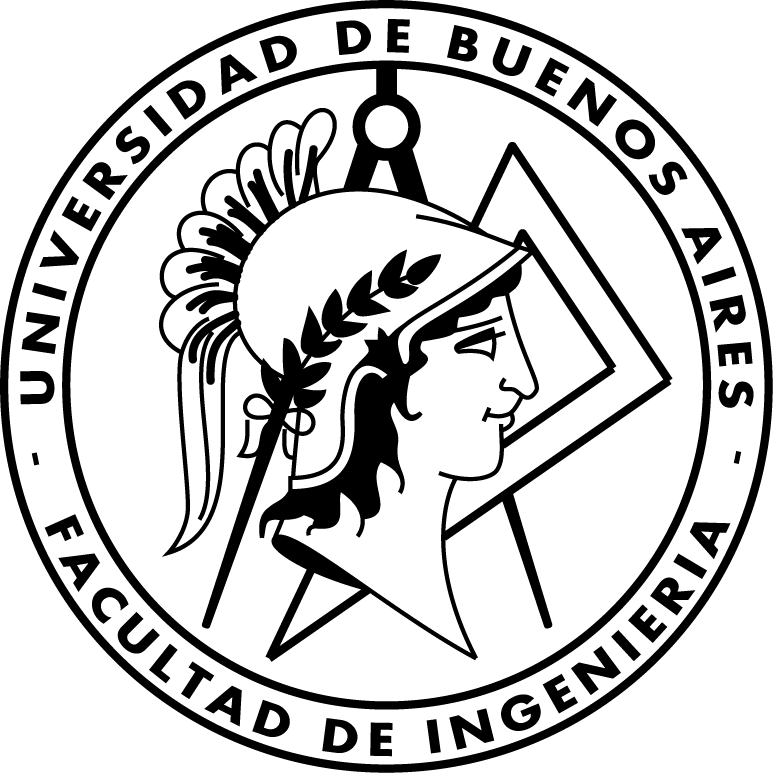
\includegraphics[scale=.4]{Logo-fiuba_big.png}

\medskip
UNIVERSIDAD DE BUENOS AIRES

Facultad de Ingenier\'ia

Departamento de Computaci\'on


\vspace{3cm}


\textbf{\large 7510 T\'ecnicas de Diseño}

\vspace{2cm}


Este es un modesto aporte para los alumnos de la f\'acultad de ingenier\'ia  de la UBA de las carreras de licenciatura en an\'alsis de sistemas e ingenier\'ia inform\'atica.
De ninguna man\'era pretende ser una gu\'ia de estudio, ni remplaza las clases presenciales, el material oficial de la catedra esta disponible en el web site de la m\'ateria.
\\
http://materias.fi.uba.ar/7510/

\end {center}


\vspace{2.5cm}

\noindent Autor:\,	Isaac Edgar Camacho Ocampo
 
\noindent Carrera:\,	Licenciatura en An\'alisis de sistemas

\vspace{1cm}

\vspace{1cm}

\noindent Buenos Aires, 2019

\newpage


\tableofcontents

\chapter{Introducción}
Toda la complejidad de la ingeniería de software surge cuando quien necesita el software ya no es quien lo construye, es decir inicialmente una persona calificada necesitaba usar la computadora para hacer algunos cálculos y demás cuestiones, entonces era el mismo quien desarrollaba el software y era el mismo quien lo usaba.

Hoy el mundo tiende a la automatización y todos los negocios están en este proceso, en general nos vamos a encontrar en la industria con la problemática de resolver algún problema, y bajo la POO el problema debe ser modelado por entidades es decir conceptos extraídos del dominio del problema.

Nosotros como analistas no somos expertos en el negocio de quien nos contrata, sin embargo debemos construir software que resuelva problemas de ese modelo de negocio, lo primero que debemos hacer es entender el negocio es decir entender las reglas de negocio que lo gobiernan.

Por ejemplo en el caso de un banco, este tendrá una linea de créditos y esta debe tener una serie de requisitos que los interesados deben cumplir,  El dueño de un restaurante debe tener reglas de negocio que dirijan la política de contratación de personal, un Supermercado tendrá reglas que determinen las disposiciones de las mercaderías en góndolas, la rotación de las mismas etc.

Así todo negocio es diferente y cuando tenemos que construir software para un negocio determinado nos enfrentamos a varios problemas.

\section{Conocimientos previos}
Aqui debo poner lo que el alumno deberia conocer


\chapter{Modelo de dominio}
Una vez que terminamos la fase de análisis de requerimientos ya sea con casos de uso o historias de usuarios, nos enfrentamos con una tarea compleja y poco clara respecto del siguiente paso en el trabajo ¿como convertir esos requisitos en el sistema funcionando es decir las lineas de código?.

Sabemos que el código surgió de un diseño previo. Pero, ¿Cómo surgió el diseño? Es decir como llego desde el modelo de casos de uso al diagrama de clases por ejemplo?
La respuesta es un modelo de análisis, hay que hacer un modelo de análisis para continuar con el trabajo.


\section{Patr\'ones de análisis (jill Nicola)}

MODELO DE ANÁLISIS 
• Objetivo: entender en detalle el negocio y sus reglas 
• Mecanismo utilizado: Patrones de Análisis 


MODELO DE DISEÑO 
• Objetivo: implementar una solución al problema planteado en el análisis más las restricciones impuestas por los requerimientos no funcionales. 
• Mecanismo utilizado: Patrones de Diseño 


Grady booch dice que tenemos como herramientas tres mecanismos.
    • PARTICIÓN: Una funcionalidad compleja dividirla en varias 
    • ABSTRACCIÓN: 
    • ESTABLECIMIENTO DE JERARQUÍAS

\chapter{Criterios de Buen Diseño SOLID}
\section{¿Qué es el criterio?} 
El criterio es nuestra herramienta para establecer diferencias y tomar decisiones, el significado de criterio es juicio o la capacidad de las personas para emitir un juicio respecto a algo o alguien de acuerdo a la información con la que cuenta. La etimología de criterio proviene del griego kriterion que significa \textbf{"norma para conocer la verdad"}.
\begin{center}
\textit{Supongamos que queremos construir una casa, ¿como empezamos? compramos materiales, llamamos a unos amigos y les decimos !!Comencemos haber que sale!!! esto seguramente es no tener criterio.
}\end{center}
\begin{center}
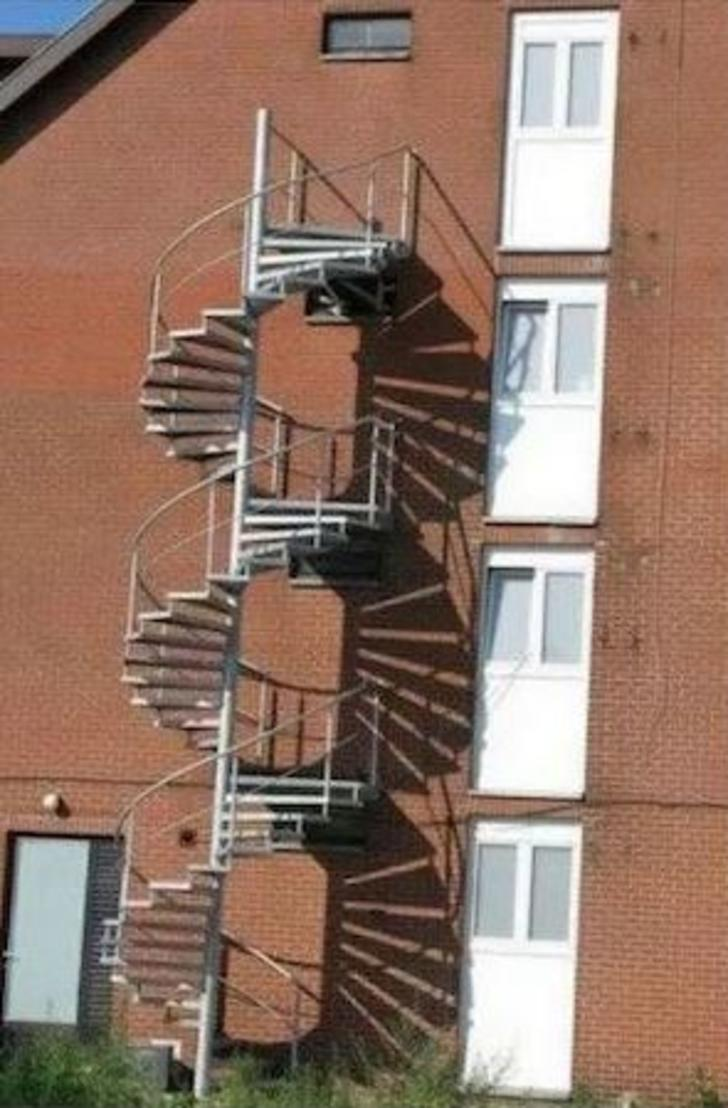
\includegraphics[scale=.3]{job3.jpg}
\end{center}
\section{Diseño}
En el artículo de Robert C. Martín \textbf{The Dependency Inversion Principle} deja en claro lo que es un mal diseño y compara el diseño de software con un trozo de carne que se va descomponiendo conforme pasa el tiempo.
\\
\\
Lo que dice el tio bob es que comparar la ingeniería del Software con la ingeniería civil es una mala comparación porque cada proyecto civil se diseña para no cambiar y la ingeniería del Software trata de modelar una porción de la realidad en la computadora, si queremos que la porción de la realidad modelada sea virtualmente parecida al mundo real, debe necesariamente cambiar, porque la naturaleza del mundo es cambiante, desde ese punto de vista la comparación con el trozo de carne que se va degradando es una buena metáfora.
\subsection{¿Que es un mal diseño?}


Estamos en presencia de un mal diseño cuando esté tiene tres cualidades.
\begin{itemize}
 \item El diseño es rígido.
 \item El diseño es frágil .
 \item Y por último el diseño es inmóvil .
 \end{itemize} Es decir las tres características de un mal diseño es la rigidez la fragilidad y la inmovilidad

\section{Diseño}



\section{Dependencia} En el campo del software una dependencia es una aplicación o una biblioteca requerida por otro programa para poder funcionar correctamente. Por ello se dice que dicho programa depende de tal aplicación o biblioteca.
\\
En UML se dice la clase A depende de la clase B.
\\
\begin{center}
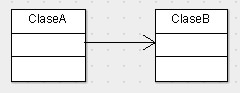
\includegraphics[scale=.5]{dependencia.png}
\end{center}
En el siguiente programa en C++ existe una dependencia con la libreria iostream.\\
\begin{center}
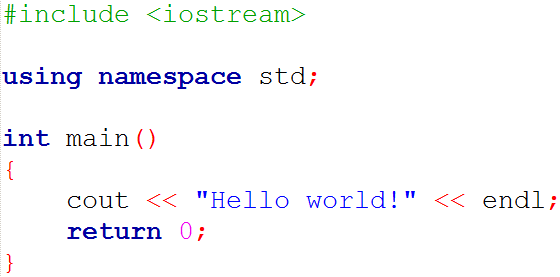
\includegraphics[scale=.5]{Hello_World_C++.png}
\end{center}

\subsection{¿Por qué preocuparse por las dependencias?}
Una dependencia es un riesgo. Por ejemplo, si mi sistema requiere la instalación de un Java Runtime Environment (JRE) y no está instalado, mi sistema no funcionará, Si un progr\'ama en lenguaje C utiliza la libreria "stdio.h" eso tambien es una dependencia y si esa libreria no esta presente ni siquiera va a compilar.
\\
Las dependencias representan riesgo y manejar ese riesgo tiene algún costo que hoy se resuelve a través de la experiencia, prueba y error, o la sabiduría colectiva de un equipo.
\subsection{¿Por que se dice inversion de las dependencias?}
En el análisis y diseño estructurados usabamos la regla de \textbf{divide y vencer\'as}, comenzamos con un problema de alto nivel y lo dividimos en partes más pequeñas. Para cualquiera de esas partes más pequeñas que todavía son "demasiado grandes", continuamos separándolas. El concepto / requisito / problema de alto nivel se divide en partes cada vez más pequeñas. El diseño de alto nivel se describe en términos de estas partes cada vez más pequeñas y, por lo tanto, depende directamente de las partes más pequeñas y más detalladas. Esto también se conoce como diseño de arriba hacia abajo.

\begin{center}
Podemos ver como el m\'odulo principal main se divide en mas funciones \\
de menor nivel y a su vez estas se vuelven a dividir, de esta manera podemos ver que\\
los modulos mas generales dependen de los detalles de implementacion.

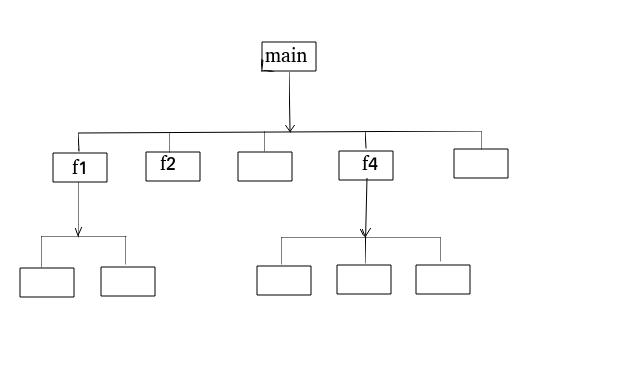
\includegraphics[scale=.7]{dis_estructur.png}
\end{center}

\begin{center}
En el Diseño orientado a objetos tanto los modulos de alto nivel, \\
como los de bajo nivel deben depender de las abstracciones.
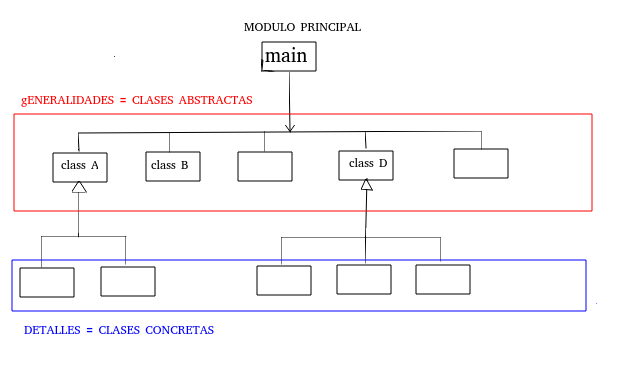
\includegraphics[scale=.7]{dis_OO.png}
\end{center}



\chapter{Parad\'igmas de Programaci\'on}
\section{Paradigma Funcional}


\chapter{Diseño de código}

\chapter{Arquitectura de Software}
\section{Introducción}
\subsection{Patrones de arquitectura}

\chapter{Temas Relacionados}
\section{Docker}
\section{API Rest}
\section{TDD}

\chapter{Patrones de Diseño}
\section{Creacioanles}
\section{De Comportamiento}

\chapter{Métricas}
\textbf{CONCEPTOS PREVIOS}
\begin{enumerate}
	\item \textbf{Eficiencia:} Producir mas con menos recursos o productividad.
	\item \textbf{Eficacia:} Lograr el resultado aunque se consuman muchos recursos.
	\item textbf{Costo de oportunidad:} Es el costo de producir una unidad de un bien.
	\item \textbf{Contribucion marginal:} Ganancia neta.
\end{enumerate}

\chapter{Conclusiones}

\textbf{CONCEPTOS PREVIOS}
\begin{enumerate}
	\item \textbf{Eficiencia:} Producir mas con menos recursos o productividad.
	\item \textbf{Eficacia:} Lograr el resultado aunque se consuman muchos recursos.
	\item textbf{Costo de oportunidad:} Es el costo de producir una unidad de un bien.
	\item \textbf{Contribucion marginal:} Ganancia neta.
\end{enumerate}
\title{\textbf{TRABAJANDO CON MODELOS MATEMATICOS LINEALES}}
\textbf{¿Que es modelizar?} Es hacer una simplificacion de la realidad y nosotros trabajamos con esa simplificacion ya que la realidad es muy compleja.
\\
\textbf{¿Para que hacer un modelo?}
\begin{itemize}
\item \textbf{Economia de recursos:} Al igual que en la ingenieria civil cuando se hacen planos para representar una obra (ya que no seria l\'ogico hacer el edificio y ante un error rehacerlo), cuando modelamos un problema usando programacion lineal y dada la escazes de recursos, es mas eficiente trabajar sobre modelos.
\item \textbf{Eficiencia}: de nuevo so no tengo recursos limitantes entonces trabajo sobre la realidad y no modelo nada.
\item \textbf{simplicidad}: puedo mediante abstracci\'on lograr un modelo mas sencillo y eliminar la complejidad inherente del problema.
\item \textbf{En resumen es mejor que hacer multiples ensayos.}
\end{itemize}
Los mod\'elos se aplican a problemas de desici\'on y este existe cuando existen formas alternativas de actuar, con distintos resultados y diferentes eficiencias para lograr el objetivo es decir existen dudas respecto del curso alternativo a utilizar.
\\
\\
\textbf{Elementos de un modelo}
\\
\\
\textbf{Hipótesis y supuestos:} Para simplificar el modelo se delimita el sistema en estudio a través de las hipótesis y
supuestos simplificativos. Así se comienza a transformar el sistema físico en un modelo simbólico.
Las hipótesis deben ser probadas científicamente. Los supuestos son hipótesis que no pueden probarse.
\\
\textbf{Ejemplos:}
Si estamos modelando una panaderia, y el recurso agua no es limitante y por otro no se dice nada de 				la venta de lo producido podemos agregar las hipotesis
\begin{enumerate}
	\item 	
	\textit{Hay agua suficiente para todos los procesos}
	\item
	\textit{Se vende todo lo que se produce}
\end{enumerate}
\textbf{Objetivo: }Mide la eficiencia de nuestro sistema y lo que buscamos es hallar la merjo solucion. El objetivo surge como respuesta a tres preguntas:
\\¿Qué hacer? es decir que es lo que queremos determinar.
\\¿Cuándo? (período de tiempo) puede ser un mes o año o un periodo t si no se especifica.
\\¿Para qué? para maximizar ganancias, o minimizar costos, nunca ambos a la vez.
\\
\\
\textbf{Actividad}
Proceso unitario que se realiza en el sistema físico caracterizado por consumir recursos
y/o generar un resultado económico y/o indicar un estado, por ejemplo producir un bien o indicar si se finaliz\'o un proceso.
\\
\\
\textbf{Variables}
Son las que miden o indican el estado de una actividad.
Las que miden pueden ser continuas o enteras.
Las que indican son, generalmente, variables (0,1) o bivalentes

\end{document}
